%!TEX root = article.tex
We report the proofs of the different propositions (\autoref{sec:proofs}), an instantiation of online Sinkhorn for discrete measures (\autoref{sec:sinkhorn_discrete}), and a supplementary experiment (\autoref{sec:supp_exp}).

We advise the reader that we provide and prove a slightly modified version of \autoref{prop:convergence}. As is, the online Sinkhorn algorithm only converges approximately, as became apparent after carefully checking our derivations. \autoref{prop:convergence} will therefore be replaced by \autoref{prop:convergence_bis} in future revisions. We provide a slight modification of the online Sinkhorn algorithm that does converge (\autoref{prop:convergence_true}). This result will be integrated to the main text in future revisions.

\section{Proofs}\label{sec:proofs}

We prove the propositions in their order of appearance.

\subsection{Proof of \autoref{prop:markov}}

\begin{proof}\todo{Why using $\infty$-norm and not the variation one?}
    We use Theorem 1 from \citet{diaconis_iterated}. For this, we simply note
    that the space $\Cc(\Xx) \times \Cc(\Xx)$ in which the chain ${x_t
    \triangleq (f_t, g_t)}_t$, endowed with the metric $\rho((f_1, g_1), (f_2,
    g_2)) = \Vert f_1 - f_2 \Vert_{\infty} + \Vert g_1 - g_2 \Vert_{\infty}$, is
    complete and separable (the countable set of polynomial functions are dense in this space, for example).
    We consider the operator $A_{\theta} \triangleq \Ctrans{\Ctrans{\cdot}{\hat
    \alpha}}{\hat \beta}$. $\theta \triangleq (\hat \alpha, \hat \beta)$ denotes
    the random variable that is sampled at each iteration. We have the following
    recursion:
    \begin{equation}
        x_{t+2} = A_{\theta_t}(x_t).
    \end{equation}
    
    For all $\hat \alpha \in \Pp(\Xx)$, $\hat \beta \in \Pp(\Xx)$, $A_{\theta}$
    with $\theta = (\hat \alpha, \hat \beta)$ is contracting, with module
    $\kappa_\theta < 1$ \citep{peyre2019computational} \todo{I have the impression $\kappa_\th<1$ should be made independend of $\theta$, which is true actually}. Therefore
    \begin{equation}
        \int_{\theta} \kappa_\theta \d \mu(\theta) < 1, \qquad \int_{\theta}
         \log \kappa_\theta \d \mu(\theta) < 0.
    \end{equation}
    Finally, we note, for all $f \in \Cc(\Xx)$
    \begin{equation}
        \Vert \Ctrans{\Ctrans{f}{\hat \alpha}}{\beta} \Vert_{\infty} 
        \leq \Vert f \Vert_\infty + 2 \max_{x,y \in \Xx} C(x, y),
    \end{equation}
    therefore $\rho(A_\theta(x_0), x_0) \leq 2 \Vert x_0 \Vert_\infty + 2
    \max_{x,y \in \Xx} C(x, y)$ for all $\theta \ (\hat \alpha, \hat \beta)$.
    The regularity condition of the theorem are therefore met. The induced Markov chains ${(f_{2t},
    g_{2t})}_t$ and ${(f_{2t + 1}, g_{2t + 1})}_t$ each have a unique stationary
    distribution. These stationary distributions are the same: the stationary distribution is independent of the initialisation and both sequences differs only by their initialisation.
    Therefore ${(f_{t}, g_{t})}_t$ have a unique stationary distribution
    $(F_\infty, G_\infty)$.
\end{proof}

\subsection{Proof of \autoref{eq:deterministic}}

The \enquote{slowed-down} Sinkhorn iterations converge toward an optimal
potential couple, up to a constant factor: this stems from the fact that we
apply contractions in the space $(\Cc(\Xx), \Vert\cdot\Vert_{\var})$ with a
contraction factor that decreases sufficiently slowly.

\begin{proof}
    We write ${(f_t, g_t)}_t$ the sequence of iterates. Given a pair of optimal potentials 
    $(f^\star, g^\star)$, we write $u_t \triangleq f_t - f^\star$, $v_t \triangleq g_t - g^\star$,
    $u_t^C \triangleq \Ctrans{f_t}{\alpha} - g^\star$ and $v_t^C \triangleq \Ctrans{g_t}{\alpha} - f^\star$
    For all $t > 0$, we observe that 
    \begin{align}
        \max u_{t+1} &= - \log \min \exp(-u_{t+1}) \\
        &= - \log \big( \min \big( (1 - \eta_t) \exp(-u_{t}) + \eta_t 
        \exp(-v_t^C) \big) \big)\\
        &\leq - \log \big( (1 - \eta_t) \min \exp(-u_{t}) + \eta_t 
        \min \exp(-v_t^C) \big)\\
        &\leq - (1 - \eta_t) \log \min \exp(-u_{t}) -  \eta_t \log \min
         \exp(-v_t^C) \\
         &= (1 - \eta_t) \max u_t  + \eta_t \max v_t^C,
    \end{align}
    where we have used the algorithm recursion on the second line, $\min f + g \geq \min f + \min g$
     on the third line and Jensen inequality on the fourth line. Similarly
    \begin{equation}
        \min u_{t+1} \geq (1 - \eta_t) \min u_t  + \eta_t \min v_t^C,
    \end{equation}
    and mirror inequalities hold for $v_t$. Summing the four inequalities, we obtain
    \begin{align}\label{eq:et}
        e_{t+1} \triangleq \Vert u_{t+1} \Vert_{\var} + \Vert v_{t+1} \Vert_{\var} 
        &= \max u_{t+1} - \min u_{t+1} + \max v_{t+1} - \min v_{t+1} \\
        &\leq
        (1 - \eta_t) ( \Vert u_t \Vert_{\var} + \Vert v_t \Vert_{\var})
        + \eta_t ( \Vert u_t^C \Vert_{\var} + \Vert v_t^C \Vert_{\var}), \\
        &\leq
        (1 - \eta_t) ( \Vert u_t \Vert_{\var} + \Vert v_t \Vert_{\var})
        + \eta_t \kappa ( \Vert u_t \Vert_{\var} + \Vert v_t \Vert_{\var}),
    \end{align}
    where we use the contractance of the soft-$C$-transform, that guarantees that
    there exists $\kappa < 1$ such that $\Vert v_t^C\Vert_{\var} \leq \kappa \Vert
    v_t\Vert_{\var}$ and $\Vert u_t^C\Vert_{\var} \leq \kappa \Vert
    u_t\Vert_{\var}$ \citep{peyre2019computational}.

    Unrolling the recursion above, we obtain
    \begin{equation}
        \log e_t = \sum_{s=1}^t \log(1 - \eta_t (1 - \kappa)) + \log(e_0) \to - \infty,
    \end{equation}
    provided that $\sum \eta_t = \infty$. The proposition follows.
\end{proof}

\subsection{Corrected version and proof of \autoref{prop:convergence}}

\makeatletter
\newcommand{\setpropositiontag}[1]{% \setpropositiontag{<tag>}
  \let\oldtheproposition\theproposition% Store \theproposition
  \renewcommand{\theproposition}{#1}% Redefine it to a fixed value
  \g@addto@macro\endproposition{% At \end{proposition}, ...
    \addtocounter{proposition}{-1}% ...restore proposition counter value and...
    \global\let\theproposition\oldtheproposition}% ...restore \thetheorem
  }
\makeatother


We make the following classic assumptions on the cost regularity and distribution compactness.

\begin{assumption}\label{ass:lip}
    The cost $C: \Xx \times \Xx \to \RR$ is $L$-lipschitz, and $\Xx$ is assumed to be compact.
\end{assumption}
As a recall, we make the following Robbins-Monroe assumptions on weights:
\begin{assumption}\label{ass:weights}
    The weight sequence ${(\eta_t)}_t$ is square summable but not summable: 
    $\sum \eta_t = \infty$ and $\sum \eta_t^2 < \infty$.
\end{assumption}
Finally, we recall that
\begin{equation}
    \Vert f \Vert_{\var} \triangleq \sup_{x \in \Xx} f(x) - \inf_{y \in \Xx} f(y).
\end{equation}

After submitting the manuscript and checking our proofs, it became apparent that a slight modification of the online Sinkhorn algorithm was needed to achieve convergence: the number of realizations used at $t$ has to be slightly increasing. We prove the following modified proposition, which establishes approximate convergence of the online Sinkhorn algorithm.

\setpropositiontag{4 bis}
\begin{proposition}\label{prop:convergence_bis}
    We assume \autoref{ass:lip} and \ref{ass:weights}. The online Sinkhorn algorithm (\autoref{alg:online_sinkhorn}) yields a sequence $(f_t, g_t)$ that reaches a
    ball centered around $f^\star, g^\star$ for the variational norm $\Vert
    \cdot \Vert_{\var}$. Namely, there exists $T > 0$, $C > 0$ such that for all $t > T$,
    \begin{equation}
        \Vert f_t - f^\star \Vert_{\var}
        + \Vert g_t - g^\star \Vert_{\var} \leq \frac{C}{\sqrt{n}} 
    \end{equation}
\end{proposition}

\begin{proof}
For discrete realizations $\hat \alpha_t$ and $\hat \beta_t$, we define the perturbation terms \todo{$\hat \alpha$ should be $\hat \alpha_t$ below?}
\begin{equation}
    \epsilon_{\hat \beta}(\cdot) \triangleq
    f^\star - \Ctrans{g^\star}{\hat \beta} ,\qquad
    \iota_{\hat \alpha}(\cdot) \triangleq 
    g^\star - \Ctrans{f^\star}{\hat \alpha},
\end{equation}
so that the updates can be rewritten as
\begin{align}
    \exp(-f_{t+1} + f^\star) &= (1 - \eta_t)
    \exp(-f_{t} + f^\star)
    + \eta_t \exp(-\Ctrans{g_t}{\hat \beta_t} 
    +\Ctrans{g^\star}{\hat \beta_t} + \epsilon_{\hat \beta_t}) \\
    \exp(-g_{t+1} + g^\star) &= (1 - \eta_t)
    \exp(-g_{t} + g^\star)
    + \eta_t \exp(-\Ctrans{f_t}{\hat \beta_t} 
    +\Ctrans{f^\star}{\hat \beta_t} + \iota_{\hat \beta_t}).
\end{align}
We denote $u_t \triangleq -f_{t} + f^\star$, $v_t \triangleq -g_{t} + g^\star$, $u_t^C \triangleq
\Ctrans{f_t}{\hat \beta_t} - \Ctrans{f^\star}{\hat \beta_t}$, $v_t^C \triangleq
\Ctrans{g_t}{\hat \beta_t} - \Ctrans{g^\star}{\hat \beta_t}$. Reusing the same
derivations as in the proof of \autoref{eq:deterministic}, we obtain
    \label{eq:pre_ineq_var}
    \begin{align}
    \Vert u_{t+1} \Vert_{\var} &\leq
    (1 - \eta_t) \Vert u_t \Vert_{\var}
    + \eta_t \log \big( \max_{x, y \in \Xx}
    \exp(\epsilon_{\hat \beta_t}(x) 
    - \epsilon_{\hat \beta_t}(y)) \exp(v_t^C(x) - v_t^C(y)) \big) \\ 
    &\leq
    (1 - \eta_t) \Vert u_t \Vert_{\var}
    + \eta_t \Vert v_t^C \Vert_{\var}
    + \eta_t \Vert \epsilon_{\hat \beta_t} \Vert_{\var},
\end{align}
where we have used $\max_x f(x) g(x) \leq \max_x f(x) \max_x f(x)$ on the second line. Therefore,
using the contractance of the soft $C$-transform,
\begin{equation}
    \label{eq:ineq_var}
    e_{t+1} \leq 
    (1 - \tilde \eta_t) e_t
    + \tilde \eta_t
    ({\Vert \epsilon_{\hat \beta_t} \Vert}_{\var} + 
    {\Vert \iota_{\hat \alpha_t} \Vert}_{\var}),
\end{equation}
where we set $e_t \triangleq \Vert u_t \Vert_{\var} + \Vert v_t \Vert_{\var}$,
$\tilde \eta_t = \frac{\eta_t}{1-\kappa}$ and $\kappa$ is set to be the minimum
of the contraction factor over all empirical realizations $\hat \alpha_t$, $\hat
\beta_t$ of the distributions $\alpha$ and $\beta$. It is upper bounded by
$1 - e^{- L\text{diam}(\Xx)}$, thanks to \autoref{ass:lip} and according to Proposition 19 in \citet{vialard2019elementary}.

The realizations $\hat \beta_t$ and $\hat \alpha_t$
are sampled according to the same distribution $\hat \alpha$ and $\hat \beta$. We
define the sequence $r_t$ to be the running average of the variational norm of the
functional error terms
\begin{equation}
    r_{t+1} = (1 - \tilde \eta_t) r_t + \tilde \eta_t 
    ({\Vert \epsilon_{\hat \beta_t} \Vert}_{\var} + 
    {\Vert \iota_{\hat \alpha_t} \Vert}_{\var}),
\end{equation}
so that we have, for all $t > 0$, $e_t \leq r_t$.
Using Lemma B.7 of
\citet{mairal_stochastic_2013} on running averages, this sequence converges towards the scalar expected value
\begin{equation}
    R = \EE_{\hat \alpha, \hat \beta}[{\Vert \epsilon_{\hat \beta} \Vert}_{\var}
    + {\Vert \iota_{\hat \alpha} \Vert}_{\var}] > 0.
\end{equation}
% The convergence occurs at the following speed: for all $t > 0$,
% \begin{equation}
%     | w_t - R | \leq C' \eta_t \sqrt{t}
% \end{equation}
We now relate $R$ to the number of samples $n$ using
a uniform law of large number result on parametric functions. We indeed have, by definition
\begin{align}\label{eq:vdv}
    \EE_{\hat \beta} {\Vert \epsilon_{\hat \beta} \Vert}_{\var} 
    &\leq
    \EE_{\hat \beta} {\Vert \Ctrans{g^\star}{\beta} 
    - \Ctrans{g^\star}{\hat \beta} \Vert}_{\infty} \\
    &= \EE_{Y_1, \dots Y_n \sim \beta} 
    \sup_{x \in \Xx}
     | \frac{1}{n} \sum_{i=1}^n \exp(g^\star(Y_i)) - C(x, Y_i))
      - \EE_{Y \sim \beta}[\exp(g^\star(Y)) - C(x, Y)] | \\
      &= \EE \sup_{x \in \Xx} | \frac{1}{n} \sum_{i=1}^n f_i(x) - f(x) | ,
\end{align}
where we have defined $f_i: x \to \exp(g^\star(Y_i - C(x, Y_i))$ and $f$ the
expected value of each $f_i$. The compactness of $\Xx$ ensures that the
functions  are square integrable and uniformly bounded. From Example 19.7 and
Lemma 19.36 of \citet{van_der_vaart_asymptotic_2000} (see also Lemma B.6 from
\citet{mairal_stochastic_2013}), there exists $C$ (that depends only on $\alpha$ and $\beta$) such that
\begin{equation}
    \EE_{\hat \beta} {\Vert \epsilon_{\hat \beta} \Vert}_{\var}  \leq \frac{C}{\sqrt{n}}.
\end{equation}
A similar results holds for $\Vert \iota_\alpha \Vert_{\var}$. The result follows by a simple comparison of sequence.
\end{proof}

\paragraph{Remark on rates.} The online Sinkhorn algorithm thus exhibits a sample complexity in
$\Oo(\frac{1}{\sqrt{n}})$ for the potential estimation. This is similar to the
batch Sinkhorn algorithm \citep{2019-Genevay-aistats}---the proof is simpler in our case, but we
assume repeated sampling.
We show in the experiment section $(\autoref{sec:exps})$ that online Sinkhorn
strongly outperforms sub-sampled Sinkhorn thanks to repeated sampling. This suggest that the constants appearing in the sample complexity bounds of online Sinkhorn are much better.

\subsection{Convergence of online Sinhkorn}

Examining the proof of \autoref{prop:convergence_bis} and in particular Eq. \eqref{eq:ineq_var}, the term that prevents the convergence of $e_t$ is the term
\begin{equation}
    \eta_t ({\Vert \epsilon_{\hat \beta_t} \Vert}_{\var} + 
    {\Vert \iota_{\hat \alpha_t} \Vert}_{\var}),
\end{equation}
which is not summable in general.
We can control this term by increasing the  size of $\hat \alpha_t$ and $\hat
 \beta_t$ with time, at a sufficient rate. This rate will be controlled by a second
 sequence ${(w_t)}_t$. Setting $n \in \NN^*$, we
 make the following assumption on the batch-sizes.

\begin{assumption}\label{ass:double_weights}
    For all $t > 0$, $\frac{n}{w_t^2}$ is an integer and the realizations
    $\hat \alpha_t$ and $\hat \beta_t$ are defined as
    \begin{equation}
         \hat \alpha_t \triangleq \frac{1}{n_{t+1} - n_t} \sum_{i=n_t}^{n_{t+1}} \delta_{x_i},
         \quad
         \hat \beta_t \triangleq \frac{1}{n_{t+1} - n_t} \sum_{i=n_t}^{n_{t+1}} \delta_{y_i},
    \end{equation}
where $(x_i)_i$ and $(y_i)_i$ are i.i.d samples of $\alpha$ and $\beta$ and
\begin{equation}
    n_{t+1} \triangleq n_t + \frac{n}{w_t^2}\quad\text{and}\quad \sum w_t
     \eta_t < \infty,\quad\text{as well as}\quad \sum \eta_t = \infty.
\end{equation}
\end{assumption}

We then have the following result of global convergence.

\begin{proposition}\label{prop:convergence_true}
    We assume \autoref{ass:lip}, and
    \ref{ass:double_weights}. Almost surely, the iterates of online Sinkhorn
    (\autoref{alg:online_sinkhorn}) converge, and we have
    \begin{equation}
        \Vert f_t - f^\star \Vert_{\var} + \Vert g_t - g^\star \Vert_{\var} \to 0.
    \end{equation}
\end{proposition}


\begin{proof}
From \eqref{eq:ineq_var}, for all $t > 0$, we have
\begin{equation}
    e_{t+1} \leq 
    (1 - \tilde \eta_t) e_t
    + \tilde \eta_t
    ({\Vert \epsilon_{\hat \beta_t} \Vert}_{\var} + 
    {\Vert \iota_{\hat \alpha_t} \Vert}_{\var}).
\end{equation}
Taking the expectation and using the uniform law of 
large number \eqref{eq:vdv}, there exists $C, C' > 0$ such that
\begin{align}
    \EE e_{t+1} &\leq (1 - \tilde \eta_t) \EE e_t + \tilde \eta_t \frac{C}{\sqrt{n_{t+1} - n_t}} \\
    &\leq (1 - \tilde \eta_t) \EE e_t + C' \tilde \eta_t w_t.
\end{align}
Writing $E_t = \EE e_t$, for all $t > 0$, $E_{t+1} - E_t \leq C' \tilde \eta_t w_t$. 
From \autoref{ass:double_weights}, ${(E_{t+1} - E_t)}_t$ is summable and $E_t \to_{t
\to \infty} \ell \geq 0$. Finally, we write
\begin{equation}
    E_T \leq E_1 - \sum_{s=1} \tilde \eta_s E_s + C\sum_{s=1} \tilde \eta_s w_s.
\end{equation}
Assuming $\ell > 0$ leads to $E_t \to -\infty$ which is absurd. Therefore $\EE
e_t \to_{t \to \infty} 0$. Since $e_t \geq 0$ for all $t > 0$, this implies that
$e_t \to_{t \to \infty} 0$ almost surely.
\end{proof}


\paragraph{Reusing past samples.}
We remark that we may also construct $\hat \alpha_t$ and $\hat \beta_t$ from $n$
fresh samples and $n (\frac{1}{w_t^2} - 1)$ previously observed samples,
without breaking the convergence proof. In this case, we still consider a stream
of samples of fixed size $(\hat \alpha_t')_t$, $(\hat \beta_t')_t$, with $n_t =
n t$, and we use it to construct $(\hat \alpha_t)_t$ and $(\hat \beta_t)_t$.

In term of algorithm, reusing samples from the past amounts to correct a fraction of the weights
$(p_i)_i$ and $(q_i)_i$ at each iteration. It is feasible provided that $\frac{1}{w_t^2} \in \Oo(t)$. The iteration complexity of the algorithm is then
$\Oo(\frac{t n^2}{w_t^2})$.

\paragraph{Examples of weights.}

Online Sinkhorn thus works for \todo{notation clash} $\eta_t = \frac{1}{n^\alpha}$ with $\alpha \in
[0, 1]$, provided we use batch-sizes of size $1 / t^{2\beta}$, with $\beta
> 1 - \alpha$. The slowing-down of Sinkhorn iterations permits to contain the
increase in the number of samples required for convergence. In particular
\begin{itemize}
    \item Setting $\eta_t = \frac{1}{t}$, the batch size can grow arbitrarily slowly ($2
    \beta > 0$ is sufficient) without breaking convergence. 
    \item Setting $\alpha = \frac{1}{2}$, the batch-size should grow linearly
    ($2 \beta = 1$) to ensure convergence. This is the limit case in which past
    samples may be reused to construct $\hat \alpha_t$ and $\hat \beta_t$.
\end{itemize}

\section{Online Sinkhorn for discrete distributions}\label{sec:sinkhorn_discrete}

The online Sinkhorn algorithm takes a simpler form when dealing with discrete
distributions. We derive it in \autoref{alg:discrete_online}. We take two
distributions of the same size for the sake of simplicity. In this case, we evaluate the potentials as
\begin{align}
    g_t(y) &= - \log \sum_{j=1}^n \exp(p_j - C(x_j, y)) \\
    f_t(x) &= - \log \sum_{j=1}^n \exp(q_j - C(x, y_j)). \\
\end{align}
Note that the computations derived in \autoref{alg:discrete_online} are proposed
in log-space so as to prevent numerical overflows. The sets $|I|$ and $|J|$ can
have varying sizes along the algorithm, which allows for example to speed-up the
initial Sinkhorn iteration (\autoref{sec:accelerating}). In such case, the
cost matrix $(C(x_i,y_j))_{i,j}$ is progressively computed along the iterations.

\begin{algorithm}[t]
    \begin{algorithmic}
    \Input Distribution $\alpha \in \triangle^n$ and 
    $\beta \in \triangle^n$, $x \in \RR^{n \times d}$, 
    $y \in \RR^{n \times d}$, learning weights ${(\eta_t)}_t$
    \State Set $p = q = - \infty \in \RR^n$
    \For{$t= 0, \dots, {T-1}$}
        \State $q \gets q + \log(1 - \eta_t)$, $p \gets p + \log(1 - \eta_t)$,
        \State Sample $I \subset [1, n]$, $J \subset [1, n]$
        \For{$i \in I$}
            \State $q_i \gets \log \big( \exp(q_i)
            + \exp(\log(\eta_t) - \log \frac{1}{n} 
            \sum_{j=1}^{n} \exp(p_j - C(x_j, y_i)) \big) $
        \EndFor
        \For{$i \in J$}
        \State $p_i \gets \log \big( \exp(q_i)
        + \exp(\log(\eta_t) - \log \frac{1}{n} 
        \sum_{j=1}^{n} \exp(q_j - C(x_i, y_j)) \big)$
        \EndFor
        \State \textit{Optional}: refit all $q_i = g_t(y_i) - \log (n)$
        \State\hspace{2.45cm} $p_i = f_t(x_i) - \log (n)$
    \EndFor
    \State Returns $f_T : (q, y)$ and
    $g_T : (p, x)$
    \end{algorithmic}
    \caption{Online Sinkhorn potentials in the discrete setting}\label{alg:discrete_online}
\end{algorithm}



\section{Experiments}\label{sec:supp_exp}

We report the performance of online+full Sinkhorn for $\epsilon \sim 10^{-4}
\max C$ in \autoref{fig:early_compute_low_eps}. Although the gains are less
important than with higher $\varepsilon$, they remain significant in this low
regularization regime.

\paragraph{Grids in \autoref{sec:exp1}.} We run the online Sinkhorn algorithm
with step-sizes \todo{notation clash} $\eta_t = \frac{1}{t^\alpha}$, $\alpha \in \{ \frac{1}{2}, 1 \}$
and $w_t = \frac{1}{{t^\beta}}$, $\beta \in \{ \frac{1}{2}, 1 \}$. In all
experiments, $\alpha = \beta = \frac{1}{2}$ turned out to perform best.

\begin{figure}[ht]
    \centering
    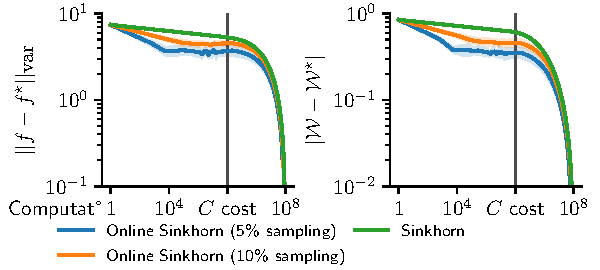
\includegraphics[width=.6\textwidth]{early_compute_low_eps.pdf}
    \caption{Online Sinkhorn accelerates the first Sinkhorn iterations even for low regularization. $\varepsilon = 10^{-4} \max C$.}
    \label{fig:early_compute_low_eps}
\end{figure}
